262. \begin{figure}[ht!]
\center{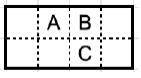
\includegraphics[scale=0.3]{rss.png}}
\end{figure}\\
На рисунке показан прямоугольник $2\times4.$ Если удалить клетки $A$ и $C$ или $B$ и $C,$ то он развалится на две части, а если удалить клетки $A$ и $B,$ то не развалится. А какое наименьшее количество клеток в прямоугольнике $5\times7$ нужно удалить, чтобы он развалился на части?\\
